\documentclass[t]{beamer}

%\documentclass[handout, t]{beamer}
\setbeamertemplate{navigation symbols}{}
\usepackage{pstricks}
\usepackage{mathtools}
\usepackage{amsfonts}
\usepackage{mathrsfs}
\usepackage{amsmath}
\usepackage{physics}
\setbeamertemplate{navigation symbols}{}
\usepackage{bm}
\usepackage[UTF8]{ctex}
\usetheme{AnnArbor}
\usefonttheme{serif}
\useinnertheme{rounded}
%\usecolortheme{beaver}
\setbeamertemplate{blocks}[rounded][shadow=true]

\newcommand{\dif}{{\;\rm d}}
\usepackage{graphicx}
\usepackage{pgf}
\usepackage{tikz}
\usetikzlibrary{arrows, decorations.pathmorphing, backgrounds, positioning, fit, petri, automata}
\tikzset{>=stealth}

\usepackage{setspace}
\setmainfont{Times New Roman}
\setCJKmainfont{Microsoft YaHei}


\hypersetup{pdfpagemode=FullScreen}
\renewcommand{\Pr}{\mathbb{P}}
\usepackage{blkarray}


\setbeamercolor{block title}{bg=red!10!white}
\setbeamercolor{block body}{bg=gray!10!white}

\usepackage{multicol}
\newcommand{\E}{\mathbb{E}}
\newcommand{\EP}{\mathbb{E}^{\mathbb{P}}}
\newcommand{\EQ}{\mathbb{E}^{\mathbb{Q}}}
\newcommand{\Var}{{\rm Var}}
\newcommand{\Cov}{{\rm Cov}}
\newcommand{\laplace}[2]{\mathcal{L}\{#1(#2)\}}
\newcommand{\LT}[1]{\mathcal{L}\{#1\}}

\begin{document}
\fontsize{11}{18}\selectfont


\CTEXindent



  \title{第六章~~更新过程}
\author{应用随机过程}
\date{中国人民大学出版社}
  \begin{frame}
    \maketitle
  \end{frame}

\begin{frame}{本章内容}
\begin{multicols}{2}
  \tableofcontents
\end{multicols}
\end{frame}


  \section{定义及例子}

  \subsection{更新过程定义}

\begin{frame}
  \frametitle{更新过程定义}
  假设$X_1,X_2,\ldots,X_n$是独立同分布的随机变量,其分布函数为$F$(为避免平凡情形,这里假设$F(0)=\Pr(X_i=0)<1,\; i=1,2,\ldots,n$),
  并且
  $$T_n=X_1+X_2+\cdots+X_n,\quad n\ge 1,\qquad T_0=0$$
  定义计数过程$N(t)=\max\{n:T_n\le t\}$,并称$N(t)$为更新过程。
  通常称$X_n$为$N(t)$的第$n$个更新间隔(inter-renewal interval),也称第$n$个更新的等待时间,称$T_n$为第$n$次更新时刻,对应的序列$\{T_n\}$称作更新序列(renewal sequence)。
  

\end{frame}


\begin{frame}
  \frametitle{更新间隔和更新时刻}
  \begin{tikzpicture}[>=stealth, thick, scale=.9]
    \draw[<->](0,5)node[right]{$N(t)$}--(0,0)--(11,0)node[below]{时间};
    \draw(0,-.1)node[below]{0}--(0,.1);
    \draw(2,-.1)node[below]{$T_1$}--(2,.1);
    \draw(3.5,-.1)node[below]{$T_2$}--(3.5,.1);
    \draw(6,-.1)node[below]{$T_3$}--(6,.1);
    \draw(9,-.1)node[below]{$T_4$}--(9,.1);
    \draw[->](10,-.1)node[below]{$t$}--(10,4)node[above]{$N(t)=4$};
    \draw[<->](0,.5)--node[fill=white]{$X_1$}(2,.5);
    \draw[<->](2,.5)--node[fill=white]{$X_2$}(3.5,.5);
    \draw[<->](3.5,.5)--node[fill=white]{$X_3$}(6,.5);
    \draw[<->](9,.5)--node[fill=white]{$X_4$}(6,.5);
    
    \draw[ultra thick](0,0)--(2,0);
    \draw[ultra thick](2,1)--(3.5,1);
    \draw[ultra thick](3.5,2)--(6,2);
    \draw[ultra thick](6,3)--(9,3);
    \draw[ultra thick](9,4)--(11,4);
    \draw[dashed](2,1)--(0,1)node[left]{1};
    \draw[dashed](3.5,2)--(0,2)node[left]{2};
    \draw[dashed](6,3)--(0,3)node[left]{3};
    \draw[dashed](9,4)--(0,4)node[left]{4};
    \draw[dashed](3.5,2)--(3.5,0);
    \draw[dashed](6,3)--(6,0);
    \draw[dashed](9,4)--(9,0);
    \draw[dashed](2,1)--(2,0);
    
    \foreach \x/\y in {2/1, 3.5/2, 6/3, 9/4}
    {
        \draw(\x,\y)[fill=black]circle(2pt);
        \draw(\x,\y-1)[fill=white]circle(2pt);
    }
    \end{tikzpicture}
  

\end{frame}    
    
    
    
    



\begin{frame}
  \frametitle{更新过程与泊松过程}
  更新过程只假设了$X_i,\; i=1,2,\ldots,n$的独立同分布(independent and identically distributed, iid),并未限定其具体服从何种概率分布;而泊松过程的定义中,则对概率分布进行了限定(指数分布)。因此,泊松过程可看作更新过程的一个特例。

  由于更新过程未限定具体的概率分布,对其的研究需要基于强大数定律的相关性质。
  

\end{frame}


\subsection{更新过程举例}

\begin{frame}
  \frametitle{举例1:马氏链}
  记$X_t$是一个不可约、正常返的离散时间马氏链,假设$X_0=x$,记$T_n$表示该马氏链第$n$次返回状态$x$的时刻。令相邻两次访问状态$x$的时间间隔为$X_i$,则有:
  \[X_i=T_{i}-T_{i-1},\qquad i=1,2,\ldots n\]
  根据强马氏性,我们可知:$X_i,\; i=1,2,\ldots n$是相互独立且同分布的,因此截至时刻$t$,访问状态$x$的次数$N(t)$就是一个更新过程,其中:$N(t)=\max\{n:T_n\le t\}$。
  

\end{frame}


\begin{frame}
  \frametitle{举例2:机器修理问题}
  一台机器在发生故障前可以正常工作的时间是$s_i$,发生故障后进行维修所花费的时间是$u_i$。记$t_i=s_i+u_i$表示机器在第$i$轮“正常工作—维修”周期的时长。若假定经维修后的机器完美如新,那么$t_i$就是独立同分布的,由此得到的截至时刻$T$,维修机器的次数$N(T)$就是一个更新过程,其中:
  $$N(T)=\max\left\{n: \left(\sum^{n}_{i=1}t_i \right) \le T\right\}$$
  
\begin{block}{说明}
  这是一种包含了“正常工作”和“维修”两个状态的交替更新过程。
\end{block}
\end{frame}


\begin{frame}
  \frametitle{举例3: $M/G/1$排队系统}
 假设有一个服务员的排队系统,顾客以速率为$\lambda$的泊松过程到达,这意味着顾客到达的时间间隔相互独立,并且服从速率为$\lambda$的指数分布。假设顾客接受服务的时间独立同分布,且均值为$\mu$。
 
 在这里我们并未假设接受服务的时间服从指数分布,因此服务时间不具有指数分布的无记忆性。
 
 对于这样的排队系统,存在“顾客到达”和“顾客接受完服务离开”两种可能的状态变化,因此该排队系统也是更新过程。
\end{frame}


\subsection{更新过程的相关术语}
\begin{frame}
  \frametitle{更新过程的相关术语}
  $N(t)$为更新过程,$X_n$为$N(t)$的第$n$个更新间隔,$T_n$为第$n$次更新时刻,则:
  \begin{enumerate}
      \item $N(t)$的期望值$M(t)$称为{\bf 更新函数}(renewal function),即:$M(t)=\E[N(t)]$;
      \item 在 $t$ 时刻,距离上一次更新的时间间隔$A(t)$称作{\bf 年龄}(age),即:$A(t)=t-T_{N(t)}$;
      \item 在 $t$ 时刻,距离下一次更新的时间间隔$Y(t)$称作{\bf 剩余寿命}(residual life),即:$Y(t)=T_{N(t)+1}-t$
  \end{enumerate}
  

\end{frame}


\begin{frame}
  \frametitle{年龄和剩余寿命}
  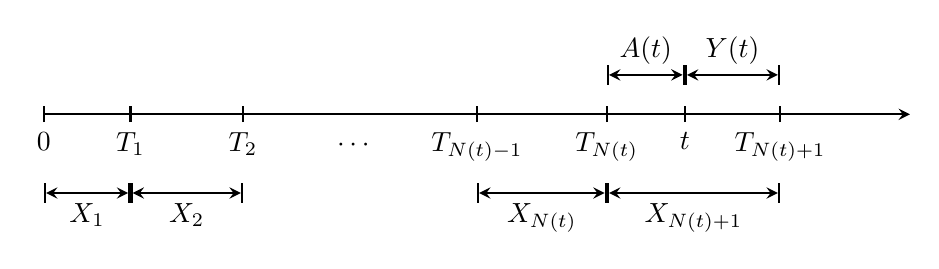
\begin{tikzpicture}[>=stealth, thick, xscale=1.1]
    \draw[->](0,0)--(10,0);
    \foreach \x/\y in {0/0,1/$T_1$,2.3/$T_2$,5/$T_{N(t)-1}$,6.5/$T_{N(t)}$,7.4/$t$,8.5/$T_{N(t)+1}$}
    {
        \draw(\x,-.1)node[below]{\y}--(\x,.1);
    }
    \node at (3.6,-.4){$\cdots$};
    \draw[|<->|](0,-1)--node[below]{$X_1$}(1,-1);
    \draw[|<->|](2.3,-1)--node[below]{$X_2$}(1,-1);
    \draw[|<->|](5,-1)--node[below]{$X_{N(t)}$}(6.5,-1);
    \draw[|<->|](6.5,-1)--node[below]{$X_{N(t)+1}$}(8.5,-1);
    \draw[|<->|](6.5,.5)--node[above]{$A(t)$}(7.4,.5);
    \draw[|<->|](7.4,.5)--node[above]{$Y(t)$}(8.5,.5);
    \end{tikzpicture}

    $A(t)$与$Y(t)$之间存在如下对应的等式关系:
\[A(t)+Y(t)=T_{N(t)+1}-T_{N(t)}=X_{N(t)+1}\]
如果图中描述的是一个电子元件的寿命,并且认为一次更新就意味着零件损坏,需要用新零件替换旧零件。$A(t)$就是零件“已经工作的时间”(年龄),$Y(t)$则是零件“还能工作多久”(剩余寿命),两者之和$A(t)+Y(t)$则表示“某个电子元件的寿命”(更新间隔)。
\end{frame}



\section{更新过程的性质}

\subsection{极限定理}
\begin{frame}
  \frametitle{极限定理}
  记$\mu=\E(X_n),\; n\ge 1$,此处的$\mu$表示更新间隔的期望值,也就是相继更新之间的平均时间。
  
  对于更新过程$N(t)$,当$n\to\infty$时,下式以概率1成立:
  \begin{equation*}
      \frac{n}{T_n}\to\frac{1}{\mu},\qquad \text{a.s.}
  \end{equation*}
  
  \begin{block}{极限定理}
    记$\mu=\E(X_n),\; n\ge 1$表示更新间隔的期望值,若$\Pr(X_i>0)>0$,那么当$t\to\infty$时,下式以概率1成立:
\begin{equation*}
    \frac{N(t)}{t}\to\frac{1}{\mu},\qquad \text{a.s.}
\end{equation*}
\end{block}
\end{frame}


\begin{frame}
  \frametitle{极限定理的图形说明}
  \begin{tikzpicture}[>=stealth, thick, scale=.9]
    \draw[<->](0,5)node[right]{$N(t)$}--(0,0)--(11,0)node[below]{时间};
    \draw(0,-.1)node[below]{0}--(0,.1);
    \draw(2,-.1)node[below]{$T_1$}--(2,.1);
    \draw(3.5,-.1)node[below]{$T_2$}--(3.5,.1);
    \draw(6,-.1)node[below]{$T_3$}--(6,.1);
    \draw(9,-.1)node[below]{$T_4$}--(9,.1);
    \draw(10,-.1)node[below]{$t$}--(10,.1)node[above]{$N(t)=4$};
    
    
    \draw(0,0)--(2,0);
    \draw(2,1)--(3.5,1);
    \draw(3.5,2)--(6,2);
    \draw(6,3)--(9,3);
    \draw(9,4)--(11,4);
    \draw[dashed](2,1)--(0,1)node[left]{1};
    \draw[dashed](3.5,2)--(0,2)node[left]{2};
    \draw[dashed](6,3)--(0,3)node[left]{3};
    \draw[dashed](9,4)--(0,4)node[left]{4};
    \draw[dashed](2,1)--(2,0);
    \draw[dashed](3.5,2)--(3.5,0);
    \draw[dashed](6,3)--(6,0);
    \draw[dashed](9,4)--(9,0);
    
    \draw[very thick](0,0)--(3,1)--(10,10/3)node[below]{$\ell_1$};
    \draw[very thick](0,0)--(5,2)--(10,4)node[right]{$\ell_2$};
    \draw[very thick](0,0)--(7,3)--(10,10*3/7)node[above]{$\ell_3$};
    \draw[dotted](3,1)--(3,0)node[below]{$t_1$};
    \draw[dotted](5,2)--(5,0)node[below]{$t_2$};
    \draw[dotted](7,3)--(7,0)node[below]{$t_3$};
    
    \foreach \x/\y in {2/1, 3.5/2, 6/3, 9/4}
    {
        \draw(\x,\y)[fill=black]circle(1.5pt);
        \draw(\x,\y-1)[fill=white]circle(1.5pt);
    }
    
    
    \end{tikzpicture}

    极限定理的含义是:当$t\to \infty$时,射线的斜率将会以概率1接近于定值$1/\mu$。
\end{frame}


\begin{frame}
  \frametitle{极限定理与泊松过程}

  泊松过程可看作更新过程的一个特例,因此若$N(t)$是泊松过程,则其更新间隔服从速率为$\lambda$的指数分布,相应$\mu=\E(X_n)=1/\lambda$
  
  当$t\to\infty$时,下式以概率1成立\[\dfrac{N(t)}{t}\to \lambda,\qquad  \text{a.s.}\]

  \begin{block}{注意:}
     $N(t)/t$反映了更新的速率,表示单位时间内更新的次数;而$t/N(t)$则反映了一次更新所需要的时间。 
  \end{block}


\end{frame}



\begin{frame}
  \frametitle{例1}
  小王的办公室有一台使用中的打印机,一旦墨盒无墨,他需要花费
  时间采购墨盒,以保证工作的顺利进行。如果打印机墨盒的寿命(天数)在区间$(60,90)$上均匀分布,小王采购墨盒需要的时间服从天数为$(1,3)$的均匀分布,那么小王应该以什么样的速率更换墨盒?
  

\end{frame}


\begin{frame}
  \frametitle{例1:解答}
 两次更换墨盒的平均时间由$\mu=\E(U_1)+\E(U_2)$得到。其中$U_1\sim U(60,90)$,$U_2\sim U(1,3)$。因此:
  \[\E(U_1)=\frac{1}{2}(60+90)=75,\qquad \E(U_2)=\frac{1}{2}(1+3)=2\]
  因此:$\mu=75+2=77$,从长远看,小王以速率1/77替换墨盒,即他需要每77天替换一次墨盒。
  

\end{frame}


\begin{frame}
  \frametitle{例2}
  假设潜在的顾客以速率为$\lambda$的泊松过程到达只有一个服务窗口的银行。假设这些潜在顾客只在服务窗口有空时才会进入银行,若银行中有一个顾客在接受服务,则潜在顾客将转身离开银行。假定进入银行的顾客在银行停留的时间是一个具有分布$G$的随机变量,则:
  \begin{enumerate}
      \item 顾客进入银行的速率是多少?
      \item 潜在的顾客最终进入银行的比例是多少?
  \end{enumerate}
  

\end{frame}


\begin{frame}
  \frametitle{例2:解答}
  记$\mu_G$为平均服务时间,根据泊松过程的无记忆性,对于进入银行的顾客而言,其时间间隔的均值$\mu$取决于到达的时间和服务的时间之和,因此
  \[\mu=\frac{1}{\lambda}+\mu_G\]
  因此进入银行的顾客速率为
  \[\frac{1}{\mu}=\frac{\lambda}{1+\lambda\mu_G}\]
  另外,由于潜在顾客到达的速率为$\lambda$,因此进入银行的顾客比例为:
  \[\frac{1/\mu}{\lambda}=\frac{\lambda/(1+\lambda\mu_G)}{\lambda}=\frac{1}{1+\lambda\mu_G}\]
  

\end{frame}


\begin{frame}
  \frametitle{}
\begin{block}{定理}
  对于更新过程$N(t)$,当$t\to\infty$,下式以概率1成立:
\[
    N(t)\to\infty,\qquad \text{a.s.} \]
\end{block}


\end{frame}


\subsection{$N(t)$的概率}
\begin{frame}
  \frametitle{$N(t)$的概率}
类似于泊松过程,在更新过程中,同样有如下等价关系成立:
  \begin{equation*}
      N(t)\ge n\quad \Longleftrightarrow \quad T_n\le t
  \end{equation*}
  于是可以得到:
  \begin{align*}
       \Pr[N(t)=n]&=\Pr[N(t)\ge n]-\Pr[N(t)\ge n+1] \\
      &=\Pr(T_n\le t)-\Pr(T_{n+1}\le t)\\
      &=F_{n}(t)-F_{n+1}(t)
  \end{align*}
  其中:$F_{n}(t)$就是$T_n$的分布函数。
  
\begin{block}{说明:}
  这个公式非常简单但难以应用,因为$F_{n}(t)$的求解往往会非常棘手。
\end{block}
\end{frame}




\begin{frame}
  \frametitle{例:}
  假设更新间隔$X_n$服从指数分布,即:
  \[F_n(t)=\Pr(X_n\le t)=1-{\rm e}^{-\lambda t}\]
由于$T_n=X_1+X_2+\cdots+X_n$服从Gamma分布,对应的概率密度函数如下:
  \[f_{T_n}(t)=\lambda {\rm e}^{-\lambda t}\cdot \frac{(\lambda t)^{n-1}}{(n-1)!},\qquad t\ge 0\]
  
  求:更新过程$N(t)$的概率$\Pr[N(t)=n]$。

\end{frame}


\begin{frame}
  \frametitle{例:解法1}
利用全概率公式可得:
  \[\begin{split}
      \Pr[N(t)=n]&=\sum_{0\le x\le t} \Pr[N(t)=n|T_n=x]\cdot \Pr(T_n=x)\\
      &= \int^t_0 \Pr[N(t)=n|T_n=x]\cdot  f_{T_n}(x)\dd x\\
      &=\int^t_0 \Pr[X_{n+1}\ge t-x] \cdot  f_{T_n}(x)\dd x\\
      &= \int^t_0 {\rm e}^{-\lambda (t-x)}\cdot \lambda {\rm e}^{-\lambda x}\cdot \frac{(\lambda x)^{n-1}}{(n-1)!}\dd x\\
      &= \frac{\lambda^n {\rm e}^{-\lambda t}}{(n-1)!}\int^t_0 x^{n-1}\dd x=\frac{\lambda^n {\rm e}^{-\lambda t}}{(n-1)!}\cdot \frac{t^n}{n} = {\rm e}^{-\lambda t}\frac{(\lambda t)^n}{n!}
  \end{split}\]
\end{frame}  

\begin{frame}{例:解法2}
利用$ \Pr[N(t)=n]=F_{n}(t)-F_{n+1}(t)$,可得:
\[\begin{split}
  F_n(t)=\Pr(T_n\le t) &= \int^t_0 f_{T_n}(s)\dd s=\int^t_0 \lambda {\rm e}^{-\lambda s}\cdot\frac{(\lambda s)^{n-1}}{(n-1)!} \dd s\\
  &=\frac{\lambda^n}{(n-1)!}\int^t_0 {\rm e}^{-\lambda s}s^{n-1}\dd s = \frac{\lambda^n}{n!}\int^t_0 {\rm e}^{-\lambda s}\dd s^n\\
\end{split}\]
其中,
\[\begin{split}
  \int^t_0 {\rm e}^{-\lambda s}\dd s^n &= {\rm e}^{-\lambda s}s^n\Big|^t_0 -\int^t_0 s^n\dd {\rm e}^{-\lambda s} \\
  &={\rm e}^{-\lambda t}t^n +\lambda \int^t_0 {\rm e}^{-\lambda s}s^n  \dd s
\end{split}\]
类似地,可得:
\[F_{n+1}(t)=\frac{\lambda^{n+1}}{(n+1)!}\int^t_0 {\rm e}^{-\lambda s}\dd s^{n+1}=\frac{\lambda^{n+1}}{n!}\int^t_0 {\rm e}^{-\lambda s}s^n\dd s\]


\end{frame}

\begin{frame}{例:解法2(cont.)}
\[\begin{split}
  \Pr[N(t)=n]&=F_{n}(t)-F_{n+1}(t)\\
  &=\frac{\lambda^n}{n!}\left[{\rm e}^{-\lambda t}t^n +\lambda \int^t_0 {\rm e}^{-\lambda s}s^n  \dd s\right]-\frac{\lambda^{n+1}}{n!}\int^t_0 {\rm e}^{-\lambda s}s^n\dd s\\
  &= {\rm e}^{-\lambda t}\frac{(\lambda t)^n}{n!}+\frac{\lambda^{n+1}}{n!}\int^t_0 {\rm e}^{-\lambda s}s^n\dd s-\frac{\lambda^{n+1}}{n!}\int^t_0 {\rm e}^{-\lambda s}s^n\dd s\\
  &= {\rm e}^{-\lambda t}\frac{(\lambda t)^n}{n!}
\end{split}\]

\begin{block}{注意:}
  最终得到的更新过程$N (t)$服从泊松分布。
\end{block}
\end{frame}





\subsection{更新函数}

\subsubsection{更新函数的性质}

\begin{frame}
  \frametitle{更新函数的性质}
  更新函数$M(t)$唯一地确定了更新过程,因此需要重点研究更新函数
  的相关性质。特别是更新间隔$X_i$的分布函数$F$与$M(t)$之间存在一一对应的关系。
  
\begin{block}{定理}
  对于分布函数$F_n(t)=\Pr(T_n\le t)$,更新函数$M(t)$满足:
  \begin{equation*}
      M(t)=\sum^{\infty}_{n=1}F_n(t)
  \end{equation*}
\end{block}

\begin{block}{说明:}
  $F_{n}(t)$的求解往往非常困难,特别是对于无穷多个$F_{n}(t)$的序列求和,通常得不到封闭表达式。因此还需要尝试使用其他的方法来求解更新函数。
\end{block}
\end{frame}


\begin{frame}
  \frametitle{}
  \begin{equation*}
    M(t)=\sum^{\infty}_{n=1}F_n(t)
\end{equation*}
  \begin{block}{证明思路}
  \begin{equation*}
    \begin{split}
        M(t)=\E[N(t)]&=\sum^{\infty}_{n=1}\Pr[N(t)\ge n]\\
    \{N(t)\ge n\}\text{与}\{T_n\le t\} \text{等价}\to   &=\sum^{\infty}_{n=1}\Pr(T_n\le t)=\sum^{\infty}_{n=1}F_n(t)\\
    \end{split}
\end{equation*}
\end{block}

\end{frame}


\begin{frame}
  \frametitle{拉普拉斯变换法求解$M(t)$}
  由于$F_n(t)$是$X_i$分布函数$F$的$n$重卷积,即:
  \begin{equation*}
      F_n(t) = \underbrace{F*F*\cdots*F}_{n\text{个}}
  \end{equation*}
  根据拉普拉斯变换的性质可知:
\[\laplace{F_n}{t}=\underbrace{\LT{F}\cdot \LT{F}\cdots \LT{F}}_{n\text{个}}=\left[\LT{F}\right]^n\]
即:$n$重卷积的拉普拉斯变换$\laplace{F_n}{t}$,可转化为分布函数$F$的拉普拉斯变换$\LT{F}$的$n$次幂。
\[    \laplace{M}{t}=\sum\limits^{\infty}_{n=1}\laplace{F_n}{t}=\sum\limits^{\infty}_{n=1}[\LT{F}]^n
\]
\end{frame}


\begin{frame}
  \frametitle{拉普拉斯变换法(cont.)}
  拉普拉斯变换法求解$M(t)$的步骤:
  \begin{enumerate}
      \item 对分布函数$F$进行拉普拉斯变换,得到$\LT{F}$;
      \item 利用$\laplace{M}{t}=\sum\limits^{\infty}_{n=1}[\LT{F}]^n$求出相应的$\laplace{M}{t}$;
      \item 对$\laplace{M}{t}$进行拉普拉斯逆变换(inverse Laplace transform),从而求出$M(t)$。
  \end{enumerate}
  

\end{frame}


\begin{frame}
  \frametitle{若干定理}
\begin{block}{定理1}
  对于$t\in [0,\infty)$,$M(t)<\infty$。
\end{block}
  
\begin{block}{推论}
  当$t=0$时,更新函数$M(t)$满足:
  \begin{equation*}
      M(0)=\frac{F(0)}{1-F(0)}
  \end{equation*}
\end{block}
\begin{block}{定理3}
  当$t\to  \infty$时,$M(t)\to \infty$
\end{block}
\end{frame}

\subsubsection{更新方程}
\begin{frame}
  \frametitle{更新方程}
  假设更新间隔$X_n$的分布函数$F$是连续的,并且有对应的密度函数$f$,则由更新函数$M(t)$构成的更新方程(renewal equation)如下:
  \begin{equation*}
      M(t)=F(t) +\int^{t}_0 M(t-x) f(x)\dd x 
  \end{equation*}
  
\begin{block}{说明:}
  更新方程提供了计算更新函数的另一种思路。
\end{block}
\end{frame}


\begin{frame}
  \frametitle{例:}
  假设更新间隔$X_n$的分布函数$F$是$[0,1]$上的均匀分布,则有:
  \[F(t)=t,\quad f(t)=1,\qquad t\in[0,1]\]

  将上式代入更新方程,可得:
  \[\begin{split}
      M(t)&=t+\int^{t}_0 M(t-x) \dd x\\
      &=t-\int^{t}_0 M(t-x)\dd (t-x)\\
      u=t-x\to &=t+\int^{t}_0 M(u)\dd u
  \end{split}\]
\end{frame}


\begin{frame}
  \frametitle{例(cont.)}
  对式子两端关于$t$求导,可得:
  \[    M'(t)=1+M(t)\]
  令$g(t)=1+M(t)$,则$g'(t)=M'(t)$,于是:
  \[g'(t) = g(t)\]
  对于这个常微分方程,易得其通解为:$g(t)=C{\rm e}^t$,相应地
  \[M(t)=C{\rm e}^t - 1\]
  由于$M(0)=\E[N(0)]=0$,因此作为初始条件可得$C=1$,最终可得:
  \[M(t)={\rm e}^t-1,\qquad t\in[0,1]\]
  

\end{frame}


\begin{frame}
  \frametitle{更新强度}
  假设更新函数$M(t)$可微,记$m(t)=\dd M(t)/\dd t$,称$m(t)$是更新函数$M(t)$对应的更新强度。
  
  \begin{block}{更新强度的性质}
    更新过程$N(t)$的更新强度$m(t)$满足:
    \begin{equation*}
        m(t)=\sum^{\infty}_{n=1}f_n(t)
    \end{equation*}
    其中:$f_n(t)$是分布函数$F_n(t)=\Pr(T_n\le t)$对应的密度函数。
    \end{block}
\end{frame}


\begin{frame}
  \frametitle{更新强度的积分方程}
  更新过程$N(t)$的更新强度$m(t)$满足如下积分方程:
  \begin{equation*}
      m(t)=f(t)+\int^t_0 m(t-x)f(x)\dd x
  \end{equation*}
  其中:$f(x)$是更新间隔$X_n$的密度函数。
  
\begin{block}{对比:更新方程}
  \begin{equation*}
    M(t)=F(t) +\int^{t}_0 M(t-x) f(x)\dd x 
\end{equation*}
\end{block}
\end{frame}


\subsubsection{更新方程与拉普拉斯变换}
\begin{frame}
  \frametitle{更新方程与卷积}
  \begin{equation*}
    M(t)=\int^t_0 f(x)\dd x+\int^{t}_0 M(t-x) f(x)\dd x 
\end{equation*}
在公式中,由于$M(t-x)$与$f(x)$的参数之和等于常数$t$,显然上式中的积分是$M(t-x)$与$f(x)$的卷积运算。

\begin{block}{拉普拉斯变换(Laplace transform)的性质}
  \begin{itemize}
    \item $\laplace{F}{t}=\dfrac{\laplace{f}{t}}{s}$
    \item $\laplace{[F*G]}{t}=\laplace{F}{t}\cdot \laplace{G}{t}$
  \end{itemize}
\end{block}
根据拉普拉斯变换的性质,更新方程可转化为:
\[    \laplace{M}{t}=\frac{1}{s}\cdot \frac{\laplace{f}{t}}{1-\laplace{f}{t}}\]
\end{frame}


\begin{frame}
  \frametitle{更新方程与拉普拉斯变换}
\[ \laplace{M}{t}=\frac{\laplace{f}{t}}{s}+\laplace{M}{t}\laplace{f}{t} \]
\begin{equation}
  \laplace{M}{t}=\frac{1}{s}\cdot \frac{\laplace{f}{t}}{1-\laplace{f}{t}}\tag{*}
\end{equation}
  
  如果求出了$f(t)$的拉普拉斯变换$\laplace{f}{t}$,并将其代入式(*),就可以得到$\laplace{M}{t}$;再对$\laplace{M}{t}$进行拉普拉斯逆变换,最终可以得到$M(t)$的表达式。
\end{frame}


\begin{frame}
  \frametitle{例:}
  假设更新过程的更新间隔密度函数如下:
  \[f(t)=\frac{1}{2}{\rm e}^{-t}+{\rm e}^{-2t},\qquad t\ge 0\]
  对其进行拉普拉斯变换,可得:
  \[\laplace{f}{t}=\frac{1}{2(s+1)}+\frac{1}{s+2}\]
  代入式(*)可得:
  \[\laplace{M}{t}=\frac{4}{3s^2}+\frac{1}{9s}-\frac{1}{9(s+1.5)}\]
  对上式进行拉普拉斯逆变换,最终可得:
  \[M(t)=\frac{4}{3}t+\frac{1}{9}\left[1-\exp\left(-\frac{3}{2}t\right)\right]\]
\end{frame}



\begin{frame}
  \frametitle{更新强度与拉普拉斯变换}
对$m(t)=f(t)+\int^t_0 m(t-x)f(x)\dd x$两端进行拉普拉斯变换,可得
\[  \laplace{m}{t}=\laplace{f}{t}+\laplace{m}{t}\laplace{f}{t}\]
对上式进行整理可得:
\begin{equation}
  \laplace{m}{t}=\frac{\laplace{f}{t}}{1-\laplace{f}{t}}\tag{**}
\end{equation}
基于式(**)的结果,对$\laplace{m}{t}$进行拉普拉斯逆变换,最终可以得到$m (t)$的表达式。
\end{frame}


\begin{frame}
  \frametitle{举例:}
  假设更新过程的更新间隔密度函数如下:
  \[f(t)=\lambda {\rm e}^{-\lambda t},\qquad \lambda>0,\; t\ge 0\]
  对其进行拉普拉斯变换,可得:$\laplace{f}{t}=\dfrac{\lambda}{\lambda+s}$

  代入式(**)可得:
  \[\laplace{m}{t}=\frac{\dfrac{\lambda}{\lambda+s}}{1-\dfrac{\lambda}{\lambda+s}}=\frac{\lambda}{s}\]
  对上式进行拉普拉斯逆变换,最终可得:$m(t)=\lambda$

\end{frame}



\subsection{更新定理}
\begin{frame}
  \frametitle{停时和瓦尔德定理}
\begin{block}{停时定义}
  假设$\{X_n\}$是随机变量序列,$S$是取值为正整数的随机变量,若$\forall n$,事件$\{S\le n\}$由$X_1,X_2,\ldots, X_n$唯一决定,则称$S$是$\{X_n\}$的停时。
\end{block}
  
\begin{block}{说明:}
  事件$\{S\le n\}$由其所在时间段的信息$X_1,X_2,\ldots, X_n$所决定。若观测到$X_1,X_2,\ldots, X_n$就能确定事件$\{S\le n\}$是否发生,则意味着$S$是停时,否则就不是。
\end{block}
\end{frame}


\begin{frame}
  \frametitle{瓦尔德定理(Wald's theorem)}
  假设$\{X_n,\; n\ge 1\}$是独立同分布的随机变量序列,其期望值均为$\mu$。$S$是定义于$\{X_n,\; n\ge 1\}$上的停时,并且$\E(S)<\infty$,则$T_S=X_1+X_2+\cdots+X_S$满足如下等式:
  \begin{equation*}
      \E(T_S)=\mu \E(S)
  \end{equation*}
\end{frame}


\begin{frame}
  \frametitle{瓦尔德定理的推论}
  瓦尔德定理可用于对更新函数$M(t)$的分析中。

  \begin{block}{推论}
    假设$\{N(t),\; t\ge 0\}$是一个更新过程,其更新间隔记作$X_i,\; i=1,2,\ldots$,对应的更新时刻记作$T_i,\; i=1,2,\ldots$。记$T_{N(t)+1}$表示$t$时刻以后的第一个更新时刻,当$\E(X_i)=\mu<\infty$时,下式成立:
\begin{equation*}
    \E[T_{N(t)+1}]=\mu [M(t)+1]
\end{equation*}
  \end{block}

\end{frame}


\begin{frame}
  \frametitle{例题:}
  某矿工身陷井下陋室。陋室有三门,他选择1号门需经过 2 天的行进才会获得自由;选择2号门则经过4 天的行进后还是回到这个陋室;选择3号门则经过 6 天的行进后还是回到这个陋室。假设在所有的时间他都等可能地选取三门中的任意一个,记这个矿工获得自由所用的时间为$T$。
\begin{enumerate}
    \item 用瓦尔德定理求$\E(T)$
    \item 计算$\E\left[\displaystyle\sum\limits^N_{i=1}X_i\Big|N=n\right]$
    \item 用(b)的结论推导出$\E(T)$
\end{enumerate}    
\end{frame}

\begin{frame}{例题:解答}
  利用瓦尔德定理,可知:$\E(T)=\E(X_i)\E(N)$,
此处$N$是停时,表示的是矿工获得自由前所做的选择次数;$X_i$表示矿工每次选择的行进天数。因此,
\[\E(X_i)=\frac{1}{3}\times \left(2+4+6\right)=4\]
需要注意的是,由于三门当中,只有1号门可以最终离开矿井,其他两门均无法离开。因此,$N$服从的是几何分布,其成功的概率为$p=1/3$,失败的概率为$2/3$。由几何分布的特征,可得:
\[\E(N)=\sum\limits^{\infty}_{n=1}n\cdot \left(\frac{2}{3}\right)^{n-1}\cdot \left(\frac{1}{3}\right)=3\]
综合上面两个式子,可得:$\E(T)=4\times 3=12$(天)。
\end{frame}

\begin{frame}{例题:解答(cont.)}
  $\{N=n\}$的含义是:前$(n-1)$次选择均未选择1号门,第$n$次选择才选择了能获得自由的1号门。因此,
\[
  \E\left[\sum\limits^N_{i=1}X_i\Big|N=n\right]=\frac{1}{2}\left(4+6\right)(n-1)+2=5n-3
\]

运用条件期望的性质,对上式两端取期望,可得:
\[\begin{split}
  \E\left\{\E\left[\sum\limits^N_{i=1}X_i\Big|N=n\right]\right\}&=5\E(N)-3\\
  \E\left[\sum\limits^N_{i=1}X_i\right]&=5\times 3-3\\
  \E(T)&=12\text{(天)}
\end{split}\]
\end{frame}





\subsubsection{基本更新定理}
\begin{frame}
  \frametitle{基本更新定理(Elementary Renewal Theorem)}

  对于更新过程$N(t)$,记$M(t)=\E[N(t)]$, $\mu=\E(X_n),\; n\ge 1$。当$t\to\infty$时,下式以概率1成立
    \begin{equation*}
        \frac{M(t)}{t}\to\frac{1}{\mu},\qquad \text{a.s.}
    \end{equation*}

    该定理是由费勒(Feller)最早提出,因此也称为费勒更新定理,其表述方式与极限定理相似,只是将$N(t)$替换成其期望$M(t)$。
  \end{frame}


  \begin{frame}
    \frametitle{极限定理与基本更新定理}
  \begin{align}
 \frac{N(t)}{t}\to\frac{1}{\mu},&\qquad \text{a.s.}\tag{极限定理}\\
      \frac{M(t)}{t}\to\frac{1}{\mu},&\qquad \text{a.s.}   \tag{基本更新定理}
  \end{align}


  极限定理的运算基于某个具体样本$\omega$下的$N(t,\omega)/t$,求解出的是时间平均更新速率(time-average renewal rate);基本更新定理对$M(t)/t$的运算,则是考虑了所有样本$\omega\in\Omega$,求解其总体的时间平均更新速率。
  
  简而言之,极限定理考查单个样本的渐近性质;基本更新定理则是考查所有样本的集成(ensemble)所具有的渐近性质。

\end{frame}


\begin{frame}
  \frametitle{举例:}
  一个工人连续干一些零活,每完成一个零活,就开始一个新的零活。每个零活需要一个具有密度函数$f$ 的随机时间独立地完成。然而会发生独立于这些的触电意外,其发生服从速率为$\lambda$的泊松过程。
  一旦发生触电意外,这个工人就不再继续手头的零活而开始一个新的。
  
  长期来看,零活完成的速率是多少?
  

\end{frame}

\begin{frame}{举例:解答}
  本问题中,将零活的完成看成一个更新过程。记更新的时间间隔为$X$,计算完成速率,需要计算出$\E(X)$。记零活完成的时间为$W$,发生触电意外的时间为$S$,则有:
\[\E(X|W=w,\; S=s)=\begin{cases}
  s+\E(X), & s<w\\
  w, & s\ge w
\end{cases}\]

\begin{block}{注意:}
  当$s<w$时,发生触电意外,此时将开始新的零活,原零活的时间$s$仍需计算在内
\end{block}
\end{frame}

\begin{frame}{举例:解答(cont.)}
  根据全概率公式可得:
  \[\begin{split}
    \E(X|W=w)&=\int^{\infty}_0 \E(X|W=w,\; S=s) \lambda {\rm e}^{-\lambda s}\dd s\\
  &=\int^w_0  [s+\E(X)]\lambda {\rm e}^{-\lambda s}\dd s  +\int^{\infty}_w w\lambda {\rm e}^{-\lambda s}\dd s\\
  &=\int^w_0 s\lambda {\rm e}^{-\lambda s} \dd s +\E(X)\int^w_0 \lambda {\rm e}^{-\lambda s}  \dd s + w\int^{\infty}_w \lambda {\rm e}^{-\lambda s}\dd s\\
  &=\left[\frac{1}{\lambda}-\left(w+\frac{1}{\lambda}\right){\rm e}^{-\lambda w}\right]+\E(X)\left(1-{\rm e}^{-\lambda w}\right)+w{\rm e}^{-\lambda w}\\
  &=\E(X)\left(1-{\rm e}^{-\lambda w}\right)+\frac{1}{\lambda}\left(1-{\rm e}^{-\lambda w}\right)\\
  &=\left[\E(X)+\frac{1}{\lambda}\right]\left(1-{\rm e}^{-\lambda w}\right)
  \end{split}\]
接下来,对上式两端取期望。
\end{frame}

\begin{frame}{举例:解答(cont.)}
由于$\E[\E(X|W=w)]=\E(X)$
,因此,
\[\begin{split}
   \E(X)&=\left[\E(X)+\frac{1}{\lambda}\right]\left[1-\E({\rm e}^{-\lambda w})\right]
   \\
   \E(X) &=\frac{1-\E({\rm e}^{-\lambda w})}{\lambda \E({\rm e}^{-\lambda w})}
\end{split}\]
因此,长期来看,零活完成的速率是$\dfrac{\lambda \E({\rm e}^{-\lambda w})}{1-\E({\rm e}^{-\lambda w})}$,其中,$$\E({\rm e}^{-\lambda w})=\int^{\infty}_0 {\rm e}^{-\lambda w}f(w)\dd w$$
\begin{block}{说明:}
  $\E({\rm e}^{-\lambda w})$是随机变量$w$的矩母函数,其参数为$-\lambda$
\end{block}
\end{frame}








\subsubsection{布莱克威尔定理}
\begin{frame}
  \frametitle{格点随机变量}
\begin{block}{定义:格点随机变量}
  若随机变量$X$只在常数$d>0$的整数倍上取值,且 
  \[\sum^{\infty}_{n=0}\Pr(X=nd)=1\]
  则称$X$是格点(lattice)随机变量。若$d$是使得上式成立的最大整数,则称$d$是$X$的周期。
\end{block}
  

\end{frame}


\begin{frame}
  \frametitle{布莱克威尔定理}
  假设$\mu=\E(X_i)$是更新过程中的平均更新间隔
  \begin{enumerate}
      \item 若$X_i$不是格点随机变量,对于$0\le a<b$,当$t\to\infty$时,
  \[M(b+t)-M(a+t)\to \frac{b-a}{\mu},\qquad 0\le a<b\]
      \item 若$X_i$是格点随机变量,且有周期$d$,当$t\to\infty$时,
      \[M(nd)-M(nd-d)\to \frac{d}{\mu},\qquad n=1,2,\ldots\]
  \end{enumerate}

  

\end{frame}

\subsection{年龄和剩余寿命}
\subsubsection{年龄和剩余寿命的长期期望值}
\begin{frame}
  \frametitle{剩余寿命$Y(t)$的展示图}
\centering
  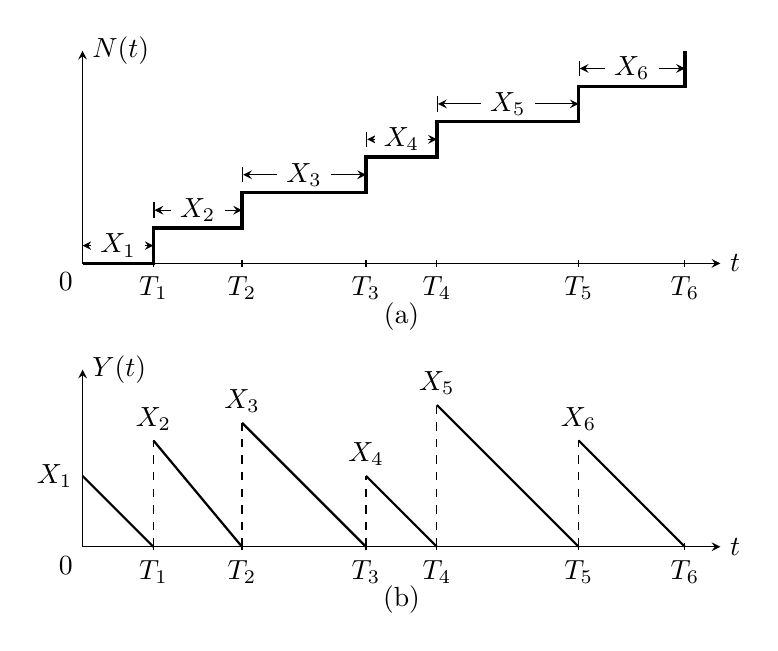
\begin{tikzpicture}[>=stealth, xscale=.9, yscale=.45]
    \begin{scope}
        \draw[<->](0,6)node[right]{$N(t)$}--(0,0)node[below left]{0}--(9,0)node[right]{$t$};
    \foreach \x/\y in {1/$T_1$, 2.25/$T_2$, 4/$T_3$, 5/$T_4$, 7/$T_5$, 8.5/$T_6$}
    {
        \draw(\x,-.1)node[below]{\y}--(\x,.1);
    }
    
    \draw[<->](0,0.5)--node[fill=white]{$X_1$}(1,.5);
    \draw[|<->](1,1.5)--node[fill=white]{$X_2$}(2.25,1.5);
    \draw[|<->](2.25,2.5)--node[fill=white]{$X_3$}(4,2.5);
    \draw[|<->](4,3.5)--node[fill=white]{$X_4$}(5,3.5);
    \draw[|<->](5,4.5)--node[fill=white]{$X_5$}(7,4.5);
    \draw[|<->](7,5.5)--node[fill=white]{$X_6$}(8.5,5.5);
    
    \draw[very thick](0,0)--(1,0)--(1,1)--(2.25,1)--(2.25,2)--(4,2)--(4,3)--(5,3)--(5,4)--(7,4)--(7,5)--(8.5,5)--(8.5,6);
    
    
    % \foreach \x/\y in {1/1, 2.25/2, 4/3, 5/4, 7/5}
    % {
    %     \draw(\x,\y)[fill=black]circle(1.5pt);
    %     \draw(\x,\y-1)[fill=white]circle(1.5pt);
    % }
    
    
    \node at (4.5,-1.5){(a)};
    
    \end{scope}
    \begin{scope}[yshift=-8cm]
        \draw[<->](0,5)node[right]{$Y(t)$}--(0,0)node[below left]{0}--(9,0)node[right]{$t$};
        \foreach \x/\y in {1/$T_1$, 2.25/$T_2$, 4/$T_3$, 5/$T_4$, 7/$T_5$, 8.5/$T_6$}
        {
            \draw(\x,-.1)node[below]{\y}--(\x,.1);
        }
    \draw[thick](0,2)node[left]{$X_1$}--(1,0);
    \draw[thick](1,3)node[above]{$X_2$}--(2.25,0);
    \draw[thick](2.25,3.5)node[above]{$X_3$}--(4,0);
    \draw[thick](4,2)node[above]{$X_4$}--(5,0);
    \draw[thick](5,4)node[above]{$X_5$}--(7,0);
    \draw[thick](7,3)node[above]{$X_6$}--(8.5,0);
    
    
    \draw[dashed](1,0)--(1,3);
    \draw[dashed](2.25,0)--(2.25,3.5);
    \draw[dashed](4,0)--(4,2);
    \draw[dashed](5,0)--(5,4);
    \draw[dashed](7,0)--(7,3);
    
    \node at (4.5,-1.5){(b)};
    \end{scope}
    \end{tikzpicture}  

\end{frame}


\begin{frame}
  \frametitle{剩余寿命$Y(t)$的长期期望值}
  研究的重点在于$t\to \infty$时,平均剩余寿命(time-average residual life)是多少。
  展示图(b)中,可以得到这些折线与横轴围成的面积$S(t)$,记作:
  \[S(t) = \int^t_0 Y(u)\dd u = \frac{1}{2}\sum^{N(t)}_{i=1}X^2_i+\int^t_{T_{N(t)}}Y(u)\dd u,\qquad t\in \left[T_{N(t)}, T_{N(t)+1}\right)\]
  平均的剩余寿命,就是$S(t)$与时间$t$的比值。根据大数定律,当$t\to\infty$时,该比率$S(t)/t\to \E[Y(t)]$

\end{frame}


\begin{frame}
  \frametitle{剩余寿命$Y(t)$的长期期望值(cont.)}
  根据夹逼定理最终可以得到:
  \begin{equation*}
    \E[Y(t)]= \lim_{t\to\infty} \frac{1}{t}\int^t_0 Y(u)\dd u=\frac{\E(X^2)}{2\E(X)},\qquad \text{a.s.}
 \end{equation*}

 平均剩余寿命的取值,取决于更新间隔$X$的一阶矩和二阶矩。
  

\end{frame}


\begin{frame}
  \frametitle{年龄$A(t)$的展示图}
  \centering
  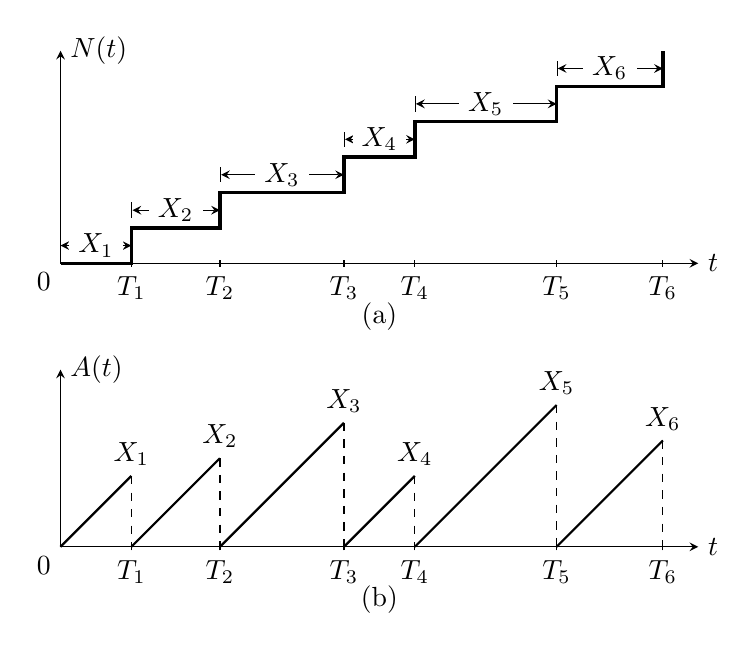
\begin{tikzpicture}[>=stealth, xscale=.9, yscale=.45]
  \begin{scope}
      \draw[<->](0,6)node[right]{$N(t)$}--(0,0)node[below left]{0}--(9,0)node[right]{$t$};
  \foreach \x/\y in {1/$T_1$, 2.25/$T_2$, 4/$T_3$, 5/$T_4$, 7/$T_5$, 8.5/$T_6$}
  {
      \draw(\x,-.1)node[below]{\y}--(\x,.1);
  }
  
  \draw[<->](0,0.5)--node[fill=white]{$X_1$}(1,.5);
  \draw[|<->](1,1.5)--node[fill=white]{$X_2$}(2.25,1.5);
  \draw[|<->](2.25,2.5)--node[fill=white]{$X_3$}(4,2.5);
  \draw[|<->](4,3.5)--node[fill=white]{$X_4$}(5,3.5);
  \draw[|<->](5,4.5)--node[fill=white]{$X_5$}(7,4.5);
  \draw[|<->](7,5.5)--node[fill=white]{$X_6$}(8.5,5.5);
  
  \draw[very thick](0,0)--(1,0)--(1,1)--(2.25,1)--(2.25,2)--(4,2)--(4,3)--(5,3)--(5,4)--(7,4)--(7,5)--(8.5,5)--(8.5,6);
  \node at (4.5,-1.5){(a)};
  
  \end{scope}
  \begin{scope}[yshift=-8cm]
      \draw[<->](0,5)node[right]{$A(t)$}--(0,0)node[below left]{0}--(9,0)node[right]{$t$};
      \foreach \x/\y in {1/$T_1$, 2.25/$T_2$, 4/$T_3$, 5/$T_4$, 7/$T_5$, 8.5/$T_6$}
      {
          \draw(\x,-.1)node[below]{\y}--(\x,.1);
      }
  \draw[thick](0,0)--(1,2)node[above]{$X_1$};
  \draw[thick](1,0)--(2.25,2.5)node[above]{$X_2$};
  \draw[thick](2.25,0)--(4,3.5)node[above]{$X_3$};
  \draw[thick](4,0)--(5,2)node[above]{$X_4$};
  \draw[thick](5,0)--(7,4)node[above]{$X_5$};
  \draw[thick](7,0)--(8.5,3)node[above]{$X_6$};
  
  \draw[dashed](1,2)--(1,0)  ;
  \draw[dashed](2.25,2.5)--(2.25,0)  ;
  \draw[dashed](4,3.5)--(4,0)  ;
  \draw[dashed] (5,2)--(5,0) ;
  \draw[dashed](7,4)--(7,0)  ;
  \draw[dashed](8.5,3)--(8.5,0);
  
  
  
  
  \node at (4.5,-1.5){(b)};
  \end{scope}
  \end{tikzpicture}
  

\end{frame}


\begin{frame}
  \frametitle{年龄$A(t)$的长期期望值}
  类似于剩余寿命的分析,可以对应得到$t\to\infty$时,平均年龄(time-average age)的取值
  \begin{equation*}
    \E[A(t)] = \lim_{t\to\infty}\frac{1}{t}\int^t_0 A(u)\dd u=\frac{\E(X^2)}{2\E(X)},\qquad \text{a.s.}
 \end{equation*}

 由于$A(t)+Y(t)=T_{N(t)+1}-T_{N(t)}=X_{N(t)+1}$,可以得到平均更新间隔(time-average interval)的结果:
\begin{equation*}
    \E[X_{N(t)+1}] =  \lim_{t\to\infty}\frac{1}{t}\int^t_{0}X_{N(u)+1}\dd u=\frac{\E(X^2)}{\E(X)},\qquad \text{a.s.}
\end{equation*}
\end{frame}


\begin{frame}
  \frametitle{总结}
  假设$X$是更新过程$N(t)$的时间间隔,且期望为$\mu$,方差为$\sigma^2$,且$X$不是格点随机变量。每次更新的年龄$A(t)$和剩余寿命$Y(t)$分别记为:
  \[A(t)=t-T_{N(t)},\qquad Y(t)=T_{N(t)+1}-t\]
  于是有:
  \begin{enumerate}
      \item $\E[Y(t)]=\dfrac{\E(X^2)}{2\E(X)}=\dfrac{\mu^2+\sigma^2}{2\mu},\qquad \text{a.s.}$
      \item $\E[A(t)]=\dfrac{\E(X^2)}{2\E(X)}=\dfrac{\mu^2+\sigma^2}{2\mu},\qquad \text{a.s.}$
      \item $\E[X_{N(t)+1}]=\dfrac{\E(X^2)}{\E(X)}=\dfrac{\mu^2+\sigma^2}{\mu},\qquad \text{a.s.}$
  \end{enumerate}
\end{frame}


\subsubsection{年龄和剩余寿命的分布}
\begin{frame}
  \frametitle{年龄$A(t)$的分布}
  具体研究当$t\to\infty$时,年龄和剩余寿命分布的渐近性质。

  先研究年龄$A(t)$的分布,假设一个系统中某个零件具有独立同分布的寿命$X_1,X_2,\ldots$。零件损坏后将立即更新,相应的更新过程记作$N(t)$。另外假设每个零件均有一个试用期$y>0$,若零件在试用期内没有损坏,则会进入正式工作期;若在试用期内损坏,则该零件将只有试用期而无正式工作期。
  
\begin{center}
  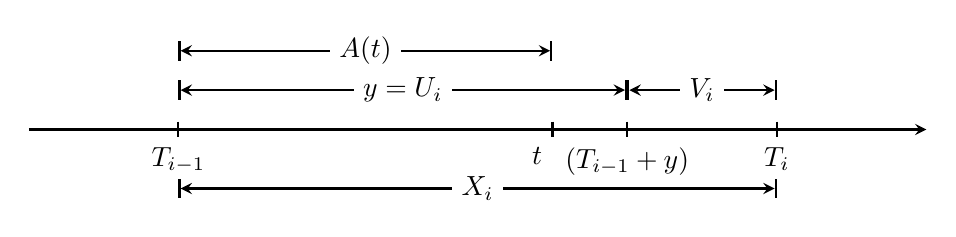
\begin{tikzpicture}[>=stealth, thick, xscale=1.9]
    \draw[->](2,0)--(8,0);
    \draw(3,0.1)--(3,-.1)node[below]{$T_{i-1}$};
    \draw(7,0.1)--(7,-.1)node[below]{$T_{i}$};
    \draw(5.5,0.1)--(5.5,-.1)node[below left]{$t$};
    \draw(6,0.1)--(6,-.1)node[below]{$(T_{i-1}+y)$};
\draw[|<->|](3,.5)--node[fill=white]{$y=U_i$}(6,.5);
\draw[|<->|](3,1)--node[fill=white]{$A(t)$}(5.5,1);
\draw[|<->|](7,.5)--node[fill=white]{$V_i$}(6,.5);
\draw[|<->|](3,-.75)--node[fill=white]{$X_i$}(7,-.75);
\end{tikzpicture}
\end{center}
\end{frame}


\begin{frame}
  \frametitle{}
  \begin{center}
    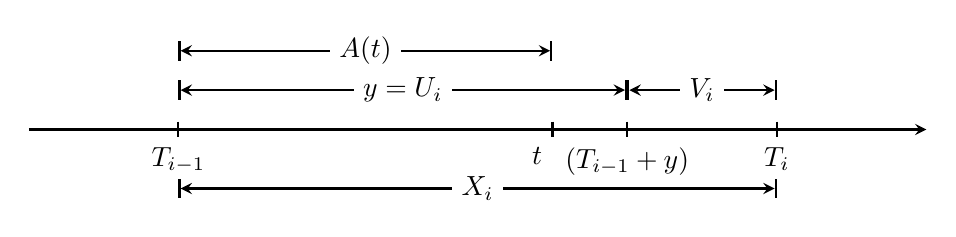
\begin{tikzpicture}[>=stealth, thick, xscale=1.9]
      \draw[->](2,0)--(8,0);
      \draw(3,0.1)--(3,-.1)node[below]{$T_{i-1}$};
      \draw(7,0.1)--(7,-.1)node[below]{$T_{i}$};
      \draw(5.5,0.1)--(5.5,-.1)node[below left]{$t$};
      \draw(6,0.1)--(6,-.1)node[below]{$(T_{i-1}+y)$};
  \draw[|<->|](3,.5)--node[fill=white]{$y=U_i$}(6,.5);
  \draw[|<->|](3,1)--node[fill=white]{$A(t)$}(5.5,1);
  \draw[|<->|](7,.5)--node[fill=white]{$V_i$}(6,.5);
  \draw[|<->|](3,-.75)--node[fill=white]{$X_i$}(7,-.75);
  \end{tikzpicture}
  \end{center}
  
  记第$i$个零件的试用期为$U_i$,则:$U_i=\min(X_i,y)$,对应的正式工作期为$V_i=X_i-U_i,\; (X_i>y)$。根据期望的性质,可得:
  \[\begin{split}
      \E(U_i) = \E[\min(X_i,y)]&=\int^{\infty}_0 \Pr[(\min(X_i,y)>s)]\dd s\\
    &=\int^y_0  \Pr(X_i>s,\; y>s)\dd s\\
   \{y>s\}\subseteq\{X_i>s\}\to   &=\int^y_0  \Pr(X_i>s)\dd s\\
      &=\int^y_0 \overline{F}(s)\dd s
  \end{split}\]
\end{frame}


\begin{frame}
  \frametitle{}
  根据强大数定律,易得:
  \[\lim_{t\to\infty}\Pr[A(t)\le y]=\frac{\E(U_i)}{\E(X_i)}\]
  由于$X_i$独立同分布,因此:$\E(X_i)=\mu$,最终可得:
  \[\lim_{t\to\infty}\Pr[A(t)\le y]=\frac{1}{\mu}\int^y_0 \overline{F}(s)\dd s,\qquad y\ge 0\]
  因此当$t$很大时,年龄$A(t)$的分布函数$ F_A(y)$可用下式近似:
  \begin{equation*}
      F_A(y)=\frac{1}{\E(X_i)}\int^y_0 \overline{F}(s)\dd s,\qquad y\ge 0
  \end{equation*}
  对上式的两端关于$y$求导,可以进一步得到$A(t)$的密度函数$f_A(y)$如下:
  \begin{equation*}
      f_A(y)=\frac{\overline{F}(y)}{\E(X_i)}=\frac{\Pr(X_i>y)}{\mu}
  \end{equation*}
  

\end{frame}


\begin{frame}
  \frametitle{剩余寿命$Y(t)$的分布}
  假设一个系统中某个零件具有独立同分布的寿命$X_1,X_2,\ldots$,相应的更新过程记作$N(t)$。零件在损坏前有一个异常状态,此状态发生在零件损坏前的$y$小时。记$V_i=\min(X_i,y)$,$U_i=X_i-V_i,\; (X_i>V_i)$。
  
\begin{center}
  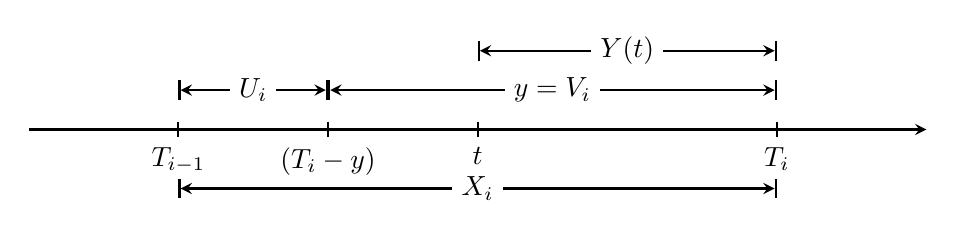
\begin{tikzpicture}[>=stealth, thick, xscale=1.9]
    \draw[->](2,0)--(8,0);
    \draw(3,0.1)--(3,-.1)node[below]{$T_{i-1}$};
    \draw(7,0.1)--(7,-.1)node[below]{$T_{i}$};
    \draw(5,0.1)--(5,-.1)node[below]{$t$};
    \draw(4,0.1)--(4,-.1)node[below]{$(T_i-y)$};
\draw[|<->|](3,.5)--node[fill=white]{$U_i$}(4,.5);
\draw[|<->|](5,1)--node[fill=white]{$Y(t)$}(7,1);
\draw[|<->|](7,.5)--node[fill=white]{$y=V_i$}(4,.5);
\draw[|<->|](3,-.75)--node[fill=white]{$X_i$}(7,-.75);
\end{tikzpicture}
\end{center}
\end{frame}


\begin{frame}
  \frametitle{}
  \begin{center}
    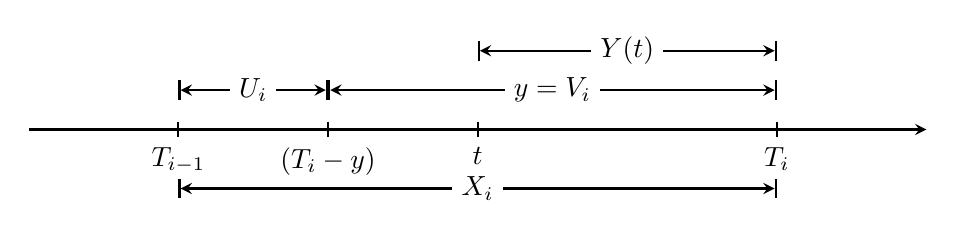
\begin{tikzpicture}[>=stealth, thick, xscale=1.9]
      \draw[->](2,0)--(8,0);
      \draw(3,0.1)--(3,-.1)node[below]{$T_{i-1}$};
      \draw(7,0.1)--(7,-.1)node[below]{$T_{i}$};
      \draw(5,0.1)--(5,-.1)node[below]{$t$};
      \draw(4,0.1)--(4,-.1)node[below]{$(T_i-y)$};
  \draw[|<->|](3,.5)--node[fill=white]{$U_i$}(4,.5);
  \draw[|<->|](5,1)--node[fill=white]{$Y(t)$}(7,1);
  \draw[|<->|](7,.5)--node[fill=white]{$y=V_i$}(4,.5);
  \draw[|<->|](3,-.75)--node[fill=white]{$X_i$}(7,-.75);
  \end{tikzpicture}
  \end{center}
  根据期望的性质,可得:
  \[
      \E(V_i) = \E[\min(X_i,y)]=\int^y_0 \overline{F}(s)\dd s
  \]
  根据强大数定律,易得:
  \[\lim_{t\to\infty}\Pr[Y(t)\le y]=\frac{\E(V_i)}{\E(X_i)}\]
\end{frame}


\begin{frame}
  \frametitle{}
  由于$X_i$独立同分布,并且$\E(X_i)=\mu$,最终可得:
  \[\lim_{t\to\infty}\Pr[Y(t)\le y]=\frac{1}{\mu}\int^y_0 \overline{F}(s)\dd s,\qquad y\ge 0\]
  因此当$t$很大时,剩余寿命$Y(t)$的分布函数$F_Y(y)$也可用下式近似:
  \begin{equation*}
      F_Y(y)=\frac{1}{\E(X_i)}\int^y_0 \overline{F}(s)\dd s,\qquad y\ge 0
  \end{equation*}
  对上式的两端关于$y$求导,可以进一步得到$Y(t)$的密度函数$f_Y(y)$如下:
  \begin{equation*}
      f_Y(y)=\frac{\overline{F}(y)}{\E(X_i)}=\frac{\Pr(X_i>y)}{\mu}
  \end{equation*}
  

\end{frame}


\begin{frame}{例题:}
  某台机器每次中断运行就换上一个同样类型的机器。如果机器的寿命服从均值为3的指数分布。
    
  请问:该机器的寿命小于一年的概率是多少?
\end{frame}


\begin{frame}
  \frametitle{例题:解法一}
本问题求解的关键在于更新过程中年龄$A(t)$的极限分布。
$X_i\sim \mathcal{E}(1/3)$,相应地,有
\[\E(X_i)=3,\qquad F(s)=\Pr(X_i\le s)=1-{\rm e}^{-\lambda s}=1-\exp\left(-\frac{1}{3}s\right)\]
因此:
\[\begin{split}
  F_A(1)=\lim_{t\to\infty}\Pr[A(t)\le 1]&=\frac{1}{\E(X_i)}\int^1_0 \overline{F}(s)\dd s\\
  &=\frac{1}{3}\int^1_0 \exp\left(-\frac{1}{3}s\right)\dd s\\
  &= -\exp\left.\left(-\frac{1}{3}s\right)\right|^1_0=1-\exp\left(-\frac{1}{3}\right)=0.283
\end{split}
  \]
  

\end{frame}

\begin{frame}
  \frametitle{例题:解法二}
根据指数分布的性质,可得:
\[\Pr(T<1)=1-{\rm e}^{-\lambda t}=1-\exp\left(-\frac{1}{3}\times 1\right)=1-\exp\left(-\frac{1}{3}\right)=0.283\]
  

\end{frame}

\section{更新过程的变化形式}

\subsection{更新奖赏过程}

\begin{frame}
  \frametitle{更新奖赏过程的定义}
  正如泊松过程是更新过程的特例,复合泊松过程可看作更新奖赏过程(renewal-reward process)的特例。
  
\begin{block}{定义}
  考虑更新间隔时间$X_n,\; n\ge 1$的更新过程$N(t)$,并假设每次更新发生时将接受一次奖赏(reward),记$R_i$为第$i$次更新时得到的奖赏,假设$R_i$独立同分布,并且$R_i$与第$i$个更新间隔$X_i$之间相互独立,则称$R(t)$为更新奖赏过程,其表达式如下:
\begin{equation*}
    R(t)=\sum^{N(t)}_{i=1}R_i
\end{equation*}
其反映了到时间$t$为止的全部奖赏数额。
\end{block}
\end{frame}


\begin{frame}
  \frametitle{}
\begin{block}{定理}
  对于更新奖赏过程$R(t)$,$R_i$为第$i$次更新时得到的奖赏,$T_i$为第$i$次更新的时间,$X_i$为第$i$个更新间隔,则下式以概率1成立:
\begin{equation*}
    \frac{R(t)}{t}\to\frac{\E(R_i)}{\E(X_i)}
\end{equation*}
\end{block}
  
\begin{block}{简要证明}
  当$t\to\infty$时,
    \[\begin{split}
        \frac{R(t)}{t}=\frac{1}{t}\sum^{N(t)}_{i=1}R_i 
        &=\frac{N(t)}{t}\cdot \frac{1}{N(t)}\sum^{N(t)}_{i=1}R_i \\
        &=\left.\frac{\sum^{N(t)}_{i=1}R_i}{N(t)}\right/\frac{t}{N(t)} \to \frac{\E(R_i)}{\E(X_i)}
    \end{split}\]
\end{block}
\end{frame}


\begin{frame}
  \frametitle{}
\begin{block}{推论}
记$\mathcal{R}(t)$是更新奖赏过程$R(t)$中的奖赏函数(reward function),其更新间隔的期望值为$\E(X)<\infty$,并且第 $i$ 次更新时得到的奖赏$R_i$满足$\E(|R_i|)<\infty$,因此:
\begin{equation*}
    \lim_{t\to\infty}\frac{1}{t}\int^t_0 \mathcal{R}(\tau)\dd \tau=\frac{\E(R_i)}{\E(X)},\qquad \text{a.s.}
\end{equation*}
\end{block}



\begin{block}{定理}
    对于更新奖赏过程$R(t)$,$R_i$为第$i$次更新时得到的奖赏,$T_i$为第$i$次更新的时间,$X_i$为第$i$个更新间隔,若$\E(R_i)<\infty$,$\E(X_i)<\infty$,则当$t\to\infty$时,下式成立:
    \begin{equation*}
        \frac{\E[R(t)]}{t}\to\frac{\E(R_i)}{\E(X_i)},\qquad \text{a.s.}
    \end{equation*}
    \end{block}
\end{frame}


\begin{frame}
  \frametitle{例1:修车问题}  
假设李师傅车的寿命是密度函数为$h$的随机变量,且如果老车损坏了就需要维修,修车需要的费用为$A$。车的寿命到达了$T$年,李师傅的车辆就需要更换,换车需要的费用为$B$。
    
  问:长期来看,李师傅在单位时间花费数额的期望值是多少?

\end{frame}


\begin{frame}
  \frametitle{例1:解答}
  对于此问题,首先要界定清楚何时修车、何时换车。假设每一次出现这样的事情经过的时间是$X_i$,假定汽车的自然寿命是$s$,那么有:
  $X_i=s\wedge T$。首先计算$\E(X_i)$:
\[\begin{split}
  \E(X_i)=\E(s\wedge T) &=\int^{\infty}_0(s\wedge T)h(s)\dd s\\
  &=\int^T_0 s h(s)\dd s +\int^{\infty}_T T h(s)\dd s\\
  &=\int^T_0 s h(s)\dd s +T\int^{\infty}_T  h(s)\dd s\\
\end{split}\]
\end{frame}


\begin{frame}
  \frametitle{例1:解答(cont.)}
对应的奖赏期望值$\E(R_i)$如下:
\[\begin{split}
  \E(R_i) &= A\cdot \Pr(s<T)+B\cdot \Pr(s\ge T)\\
  &=A\int^T_0 h(s)\dd s+B\int^{\infty}_T h(s)\dd s
\end{split}\]
因此:单位时间花费数额的期望值是
\[\frac{\E(R_i)}{\E(X_i)}=\frac{\displaystyle  A\int^T_0 h(s)\dd s+B\int^{\infty}_T h(s)\dd s}{\displaystyle  \int^T_0 s h(s)\dd s +T\int^{\infty}_T  h(s)\dd s}\]
  

\end{frame}


\begin{frame}
  \frametitle{例2:火车发车问题}
  假设旅客按间隔时间的均值为$\mu$的更新过程到达火车站。一旦有$N$位旅客等候,就发出一列火车。如果火车站有$n$个旅客在等待,会引起单位时间$nc$元的费用。

问:火车站单位时间产生的平均费用是多少?

\begin{block}{提示:}
  该问题中,发出一列火车,就意味着完成一次更新,而一次更新的时间间隔,就会发生因旅客等待而产生的费用,这些费用可看成“奖赏”,在更新发生的时间间隔产生。因此该问题属于更新奖赏过程。
\end{block}
\end{frame}


\begin{frame}
  \frametitle{例2:解答}
  由于到达时间间隔的均值是$\mu$,只有当等待的旅客数凑够$N$人才会触发更新,因此:
  \[\E(X_i)= N\cdot\E(T_i) =  N\cdot \mu\]
  记$T_n$表示第$n$位到达的旅客与第$(n+1)$位到达的旅客之间的时间间隔,于是:
  \[\E(R_i)=\E[c\cdot T_1+2c\cdot T_2+\cdots +(N-1)c\cdot T_{N-1}]\]
  由于$\E(T_i)=\mu$,因此:
  \[\E(R_i)=c[\mu+2\mu+\cdots+(N-1)\mu]=c\mu\frac{N(N-1)}{2}\]
  因此火车站单位时间产生的平均费用是:
  \[\frac{\E(R_i)}{\E(X_i)}=\frac{c\mu N(N-1)}{2N\mu}=\frac{c(N-1)}{2}\]
\end{frame}

\subsection{交替更新过程}

\begin{frame}
  \frametitle{交替更新过程的定义}
    假设在状态1下,$s_1,s_2,\ldots$独立同分布,且分布函数为$F$,期望值为$\mu_F$;假设在状态2下,$u_1,u_2,\ldots$独立同分布,且分布函数为$G$,期望值为$\mu_G$,并且这两组随机变量之间是交替的。由此所得到的更新过程$N(t)$称为交替更新过程(alternating renewal process)。

    \begin{center}
      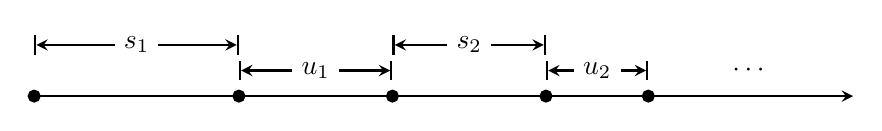
\begin{tikzpicture}[>=stealth, thick, scale=1.3]
        \draw[->](0,0)--(8,0);
        \foreach \x in {0,2,3.5,5,6}
        {
            \draw[fill=black](\x,0) circle (1.5pt);
        }
        \draw[|<->|](0,.5)--node[fill=white]{$s_1$}(2,.5);
        \draw[|<->|](3.5,.25)--node[fill=white]{$u_1$}(2,.25);
        \draw[|<->|](3.5,.5)--node[fill=white]{$s_2$}(5,.5);
        \draw[|<->|](5,.25)--node[fill=white]{$u_2$}(6,.25);
        \node at (7,.25){$\cdots$};
    \end{tikzpicture} 
    \end{center}
\end{frame}


\begin{frame}
  \frametitle{}  
\begin{block}{定理}
  在一个交替更新过程中,处于状态1的时间所占比例的极限为
  $\dfrac{\mu_F}{\mu_F+\mu_G}$
\end{block}

\begin{block}{证明思路1}
  可以将状态1看作“开”(on),将状态2看作“关”(off)。一次更新伴随着“开”—“关”循环(on-off cycle)一次。那么处于状态1的时间所占比例,可以看作系统处于“开”的平均时间占总时间的比例。因此根据大数定律,该比例可以记为:
\begin{equation*}
       \frac{\E(\text{“开”状态的时间})}{\E(\text{总时间})}=
    \frac{\E(\text{“开”状态的时间})}{\E(\text{“开”状态的时间})+\E(\text{“关”状态的时间})}
\end{equation*}
于是可得:
\[\frac{\E(R_i)}{\E(X_i)}=\frac{\mu_F}{\mu_F+\mu_G}\]
\end{block}

  

\end{frame}


\begin{frame}
  \frametitle{证明思路2}
\begin{center}
  \begin{tikzpicture}[>=stealth, thick, scale=1.2]
    \draw[->](0,0)--(8,0);
    \foreach \x in {0,2,3.5,5,6}
    {
        \draw[fill=black](\x,0) circle (1.5pt);
    }
    \draw[|<->|](0,.4)--node[fill=white]{$s_1$}(2,.4);
    \draw[|<->|](3.5,.4)--node[fill=white]{$u_1$}(2,.4);
    \draw[|<->|](3.5,.4)--node[fill=white]{$s_2$}(5,.4);
    \draw[|<->|](5,.4)--node[fill=white]{$u_2$}(6,.4);
    \node at (7,.4){$\cdots$};
    \node at (2,-.4){$s_1$};
    \node at (5,-.4){$s_2$};
    \node at (6,-.4){$0$};
    \node at (3.5,-.4){$0$};
    \node at (0,-.4){$0$};
\node at (-1,.4){时间};
\node at (-1,-.4){奖赏};
\end{tikzpicture}
\end{center}

  将相邻的两个时间段进行两两分组,并且如果处于状态1,就在状态1到达的时候记录一个奖赏$s_i$,表示处于状态1的时间$s_i$。否则就记奖赏为0。于是可得:
\[\E(R_i)=\E(s_i)=\mu_F,\qquad \E(X_i)=\E(s_i)+\E(u_i)=\mu_F+\mu_G\]
根据更新奖赏过程的结论,可得:
\[\frac{R(t)}{t}\to \frac{\E(R_i)}{\E(X_i)}=\frac{\E(s_i)}{\E(s_i)+\E(u_i)}=\frac{\mu_F}{\mu_F+\mu_G}\]

\end{frame}


\begin{frame}
  \frametitle{例1:机场接站问题}
  假设某机场的国际航班出站旅客的分布服从一个速率为每小时10人的泊松过程,有一辆面包车,它每接满7人就会立刻出发,送这批旅客前往位于市区的酒店。36分钟之后,这辆面包车就会回来。如果到达的旅客没有看到面包车,就会自行前往机场附近的酒店。

  请问:长时间来看,多少比例的旅客最终会去市区的酒店?
\end{frame}


\begin{frame}
  \frametitle{例1:解答}
  假设$s_i$表示面包车接旅客,在机场停留的时间;$u_i$表示在面包车从离开机场到回到机场花费的时间(本问题中,此值为常数36分钟,即$0.6$小时),于是可得:
  \[\E(s_i)=\frac{1}{10}\times 7=0.7,\qquad \E(u_i)=0.6\]
  最终去市区酒店的旅客比例为:
  \[\frac{\E(s_i)}{\E(s_i)+\E(u_i)}=\frac{0.7}{0.7+0.6}=\frac{7}{13}\]
  

\end{frame}


\begin{frame}
  \frametitle{例2:换灯泡问题}
  假如灯泡寿命的分布函数为$F$,均值为$\mu_F$。一个修理工会不定期来检查灯泡,检查灯泡的时间服从一个速率为$\lambda$的泊松过程。如果发现灯泡坏了,就会立即更换。求:
  \begin{enumerate}
  \item 灯泡更换的速率。
  \item 长期来看,灯泡正常工作的时间占比。
  \item 长期来看,修理工检查灯泡的时候不用更换灯泡的次数占比。
  \end{enumerate}
  
\begin{block}{思路}
  假设在0时刻安上一个新灯泡,它将持续工作的时间长度为$s_1$,根据指数分布的无记忆性,到下次检查灯泡还需要经过的时间长度为$u_1$,相应的$u_1$时长服从速率为$\lambda$的指数分布,依此类推开始新的更新周期。从中不难看出,这是一个交替更新过程。  
\end{block}
\end{frame}


\begin{frame}
  \frametitle{例2:解答}
  (1) 每次更新的时间间隔期望值$\E(X_i)$取决于灯泡工作时间和检查灯泡的时间间隔之和,因此:
  \[\E(X_i)=\frac{1}{\lambda}+\mu_F\]
  根据极限定理,可得:
  \[\frac{N(t)}{t}\to \frac{1}{\E(X_i)}=\frac{1}{\mu_F+1/\lambda}\]
  因此,需要平均$\mu_F+1/\lambda$的时间更换一次灯泡。
  
  (2) 令$R_i=s_i$,于是可得:
  \[\frac{\E[R(t)]}{t}\to \frac{\E(R_i)}{\E(X_i)}=\frac{\mu_F}{\mu_F+1/\lambda}\]
  灯泡正常工作的时间占比为$\mu_F/(\mu_F+1/\lambda)$
  

\end{frame}


\begin{frame}
  \frametitle{例2:解答(cont.)}
  (3) 假设截至$t$时刻,修理工来访了$V(t)$次,相应修理工换了$N(t)$次灯泡。于是本问题我们需要计算的就是:
  \[\frac{V(t)-N(t)}{V(t)}=1-\frac{N(t)}{V(t)}\]
  由于修理工检查灯泡的时间服从速率为$\lambda$的泊松过程,因此:
  \[\frac{V(t)}{t}\to \lambda\]
  另外,结合(1)中得到的结果可得:
  \[\frac{V(t)-N(t)}{V(t)}=1-\frac{N(t)}{V(t)}=1-\left[\frac{N(t)}{t}\left/\frac{V(t)}{t}\right. \right]\to 1-\frac{1}{\lambda \mu_F+1}=\frac{\mu_F}{\mu_F+1/\lambda}\]
  

\end{frame}




\end{document}